\chapter{Solidity static analysis methods}

Solidity already benefits from in-built static analysis tools and a compiler, ${solc}$. Some of the optimizations already done are well documented, as per Solidity's official documentation \cite{solidity-documentation}.

In this chapter, we'll go over some of the external tools built for Solidity optimization, as the main objective for this thesis is to extend, enhance and/or build such tools, as an improvement over the existing official toolkit.

\section{Solidity Instrumentation Framework (SIF)}

Built by Chao Peng, Sefa Akca and Ajitha Rajan, from University of Edinburgh, SIF is a tool built in C that gravitates around the Visitor Design Pattern. The main objective is to build an internal C representation of Solidity code, through intermediary data structures, upon which SIF can orchestrate various optimizations / refactoring functions. As the authors describe it, it's a tool "to easily and effectively understand, manipulate and analyse Solidity code" \cite{sif}.

The drawbacks that this toolkit currently have is that it's outdated and that it does not allow for external users to "plug-in" their own intermediate representations of Solidity code. It acts more as a middle-man, allowing users to implement, through the \emph{visit} method, specific optimization / refactoring items that run against isolated pieces of code. The tool does build a Control Flow Graph for the code, the one that this thesis will focus on, but it does not specifically use it for any kind of in-house optimization – it is just available to the user for usage.

\section{Slither}

Slither is a more abstract, high level static analysis framework, which gives a broader overview over the internals of an Ethereum smart contract. Its main focus is centered around 4 areas: security (vulnerability detection), automated code optimization, code analysis and assisted code review, as described in Section 4.1 by the author Margherita Renieri \cite{slither}.

The tool takes advantage of the Abstract Syntax Tree (AST) built by the Solidity Compiler, then passes that through a series of optimization steps: Information Recovery, SlithIR conversion and Code analysis.

What's common in both of the tools we've seen is the usage of Abstract Syntax Trees and Control Flow Graphs, as well as building "proprietary" intermediate representation of the input code.

\begin{figure}
    \centering
    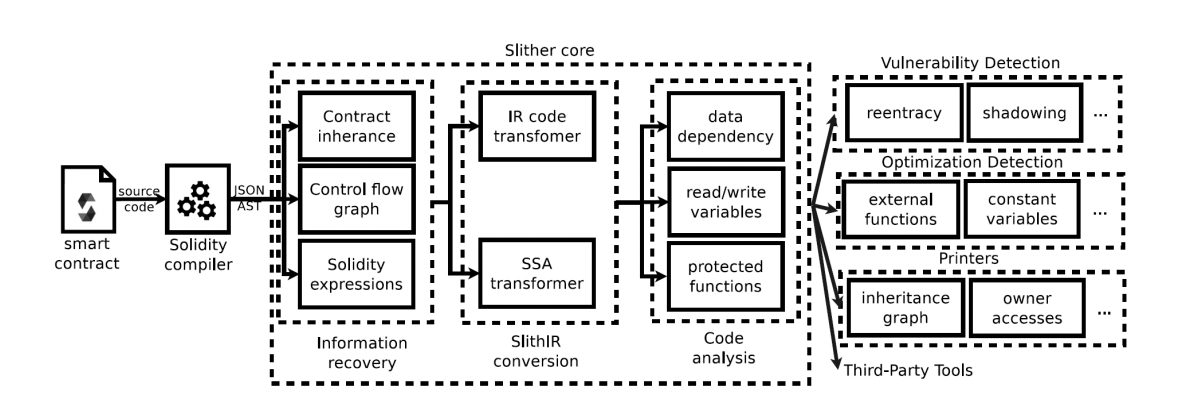
\includegraphics[width=15cm]{images/slither_architecture.png}
    \caption{Slither Architecture}
    \label{fig:slither-architecture}
\end{figure}